% --------------------------------------------
% Chapter 3 — Force Main Design and Hydraulic Assessment
% --------------------------------------------

\section{Force Main Design and Hydraulic Assessment}


% -------------------------------------------------
% 3.0 Force Main Layout and System Configuration
% -------------------------------------------------
\subsection{Layout and System Configuration}

The physical configuration of the wastewater conveyance system was first established in order to determine the hydraulic parameters required for the pump station design. The system consists of a submersible lift station located within the Colebrooke Subdivision that conveys wastewater through a short force main to an existing city gravity sewer manhole. The geometric layout of the force main, including stationing, pipeline length, and connection points, was developed using Autodesk Civil 3D 2025.

The alignment of the pipeline was created using the \textit{Alignment} tools within Civil 3D, while the force main was modeled using the \textit{Pipe Network} tools to define pipe size, slope conditions, and the connection to the downstream manhole. This modeling process allowed accurate extraction of the pipeline length, elevations, and spatial relationships required for the hydraulic calculations performed in the following sections.

The resulting plan layout of the proposed force main and pump station is illustrated in Figure~\ref{fig:force_main_plan}. The drawing identifies the location of the pump station, the beginning and ending station of the force main, and the receiving city sewer manhole. The force main extends approximately $77.48~\text{ft}$ from the pump station to the receiving manhole where the wastewater discharges into the existing gravity sewer system. The drawing also provides key survey coordinates and elevation information used to establish the hydraulic profile of the system.

\begin{figure}[H]
\centering
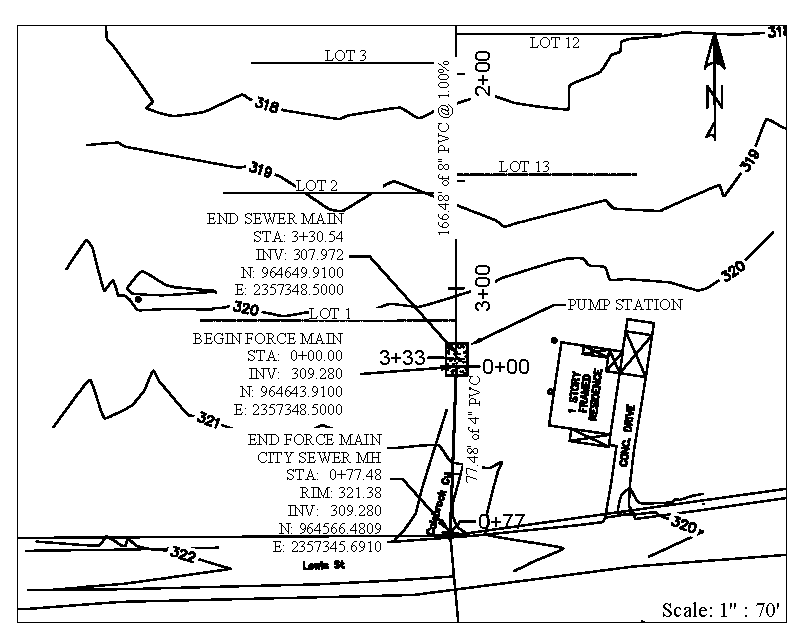
\includegraphics[
width=\textwidth,
]{ForcemainLayoutPlan.pdf}
\caption{Force main layout plan showing pump station location, pipeline alignment, and connection to the city sewer manhole.}
\label{fig:force_main_plan}
\end{figure}

The hydraulic relationship between the wet well and the receiving gravity sewer is illustrated in Figure~\ref{fig:pump_station_profile}. The profile diagram shows the wet well operating elevations, the discharge elevation at the receiving manhole, and the approximate length of the force main connecting the two structures. The wet well receives an inflow of $12.46~\text{gpm}$, and wastewater is conveyed through the force main to the downstream manhole located at an elevation of $309.28~\text{ft}$. These elevations define the vertical difference that produces the static head component used in the total dynamic head calculations.

\begin{figure}[H]
\centering
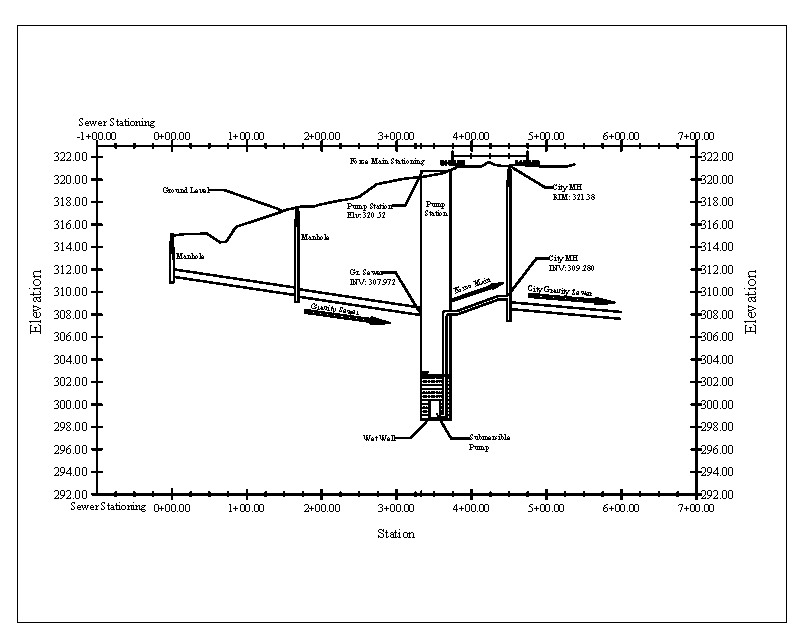
\includegraphics[
width=\textwidth,
trim={0.3in 0.6in 0.4in 0.6in},
clip
]{ForceMainLayoutProfile.pdf}
\caption{Hydraulic profile of the pump station showing wet well elevations, force main length, and discharge elevation at the receiving manhole.}
\label{fig:pump_station_profile}
\end{figure}

The plan and profile drawings provide the geometric basis for the hydraulic design of the system. The pipe length obtained from the Civil 3D alignment model, together with the discharge elevation and wet well water surface elevation, forms the basis for determining static head, friction losses, and minor losses in the force main. These parameters are used in the following sections to develop the system head requirements and establish the system curve for pump selection in accordance with the methodology described in the Jensen pump station design guidelines~\cite{ProjectD_Colebrooke_2020}.



% -------------------------------------------------
% 3.1 Force Main Material Selection
% -------------------------------------------------
\subsection{Force Main Material Selection}

The pressure pipeline connecting the proposed pump station to the downstream municipal sewer manhole functions as a force main that conveys wastewater under pressurized conditions. Selection of an appropriate pipe material is therefore an important design consideration because the material directly influences hydraulic performance, durability, constructability, and long-term operational reliability of the wastewater conveyance system.

For the Colebrooke Subdivision system, polyvinyl chloride (PVC) pressure pipe is selected as the force main material. PVC pipe is commonly used in wastewater conveyance applications due to its corrosion resistance, smooth internal surface, and relatively low installation cost compared with metallic pipe alternatives. The material is lightweight and relatively easy to install, which is advantageous for short pipeline segments such as the approximately 77.48~ft force main required for this project. These characteristics make PVC pipe a practical and reliable option for small lift station installations serving residential developments.

The selection of PVC pipe for the force main was made in consultation with applicable wastewater infrastructure guidance and pump station design references. Regulatory design guidance for publicly owned wastewater facilities recommends materials that provide corrosion resistance and long-term durability in sanitary sewer environments~\cite{MDEQ_DesignGuidance_2025}. In addition, pump station design practices described in the Jensen pump station design guidelines recognize PVC pressure pipe as a commonly used material for wastewater force mains due to its favorable hydraulic characteristics and ease of construction~\cite{Jensen_PumpStationDesignGuidelines_2012}.

A key hydraulic advantage of PVC pipe is its relatively smooth interior surface, which reduces friction losses during pressurized flow. In hydraulic analysis using the Hazen--Williams equation, this smoothness is represented by the Hazen--Williams roughness coefficient \(C\). For the PVC force main considered in this design, the following value is adopted:

\[
C = 135
\]

This value is consistent with commonly used design coefficients for new PVC pressure pipes and is suitable for evaluating friction losses in wastewater force mains using the Hazen--Williams formulation~\cite{Jensen_PumpStationDesignGuidelines_2012}. The selected roughness coefficient will be used in subsequent sections to estimate friction head losses within the force main during system operation.


% -------------------------------------------------
% 3.2 Force Main Diameter
% -------------------------------------------------
\subsection{Force Main Diameter}

An initial evaluation of the force main diameter was performed using the design flow provided by the sewer design team,
$Q = 12.46 \ \text{gpm}$.

The objective of this step is to evaluate the hydraulic performance of different pipe diameters and verify whether the resulting flow velocity satisfies typical wastewater force main velocity criteria.

The initial assumptions used for the preliminary hydraulic evaluation are summarized in Table~\ref{tab:diameter_inputs}.

\begin{table}[H]
\centering
\caption{Hydraulic Evaluation Parameters}
\label{tab:diameter_inputs}
\begin{tabular}{lll}
\toprule
\textbf{Parameter} & \textbf{Value} & \textbf{Unit} \\
\midrule
Design flow, $Q$ & 12.460 & gpm \\
Wet well water surface & 299.000 & ft \\
City sewer invert & 309.280 & ft \\
Static head, $H_s$ & 10.280 & ft \\
Force main length, $L$ & 77.480 & ft \\
Hazen--Williams coefficient, $C$ & 135 & -- \\
Total loss coefficient, $K$ (check + gate + bends + exit) & 5.100 & -- \\
Gravity, $g$ & 32.200 & ft/s$^2$ \\
Pump efficiency, $\eta$ & 0.60 & -- \\
\bottomrule
\end{tabular}
\end{table}

These parameters establish the baseline conditions used to evaluate candidate pipe diameters.

\subsubsection*{Hand Calculation Example (1-in Pipe)}

To demonstrate the procedure used in evaluating the force main diameter, a detailed hand calculation is presented for the case of a 1-inch diameter pipe.

\textbf{Convert Flow Rate}

The design flow must first be converted from gallons per minute to cubic feet per second.
\[
  \begin{aligned}
    & Q = 12.46 \ \text{gpm} \\
    &\Rightarrow Q = 12.46 \times \frac{1 \ \text{ft}^3}{7.48 \ \text{gal}} \times \frac{1}{60}\\
    &\therefore Q = 0.0278 \ \text{ft}^3/\text{s}
  \end{aligned}
\]


\textbf{Pipe Area}

For a 1-inch inside diameter pipe,
$D = 1 \ \text{in} = \frac{1}{12} \ \text{ft} = 0.0833 \ \text{ft}$

The pipe cross-sectional area is
\[
  \begin{aligned}
    & A = \frac{\pi D^2}{4} \\
    &\Rightarrow A = \frac{\pi (0.0833)^2}{4}\\
    &\therefore A = 0.0055 \ \text{ft}^2
  \end{aligned}
\]


\textbf{Velocity}

Velocity is calculated using the continuity equation:

\[
  \begin{aligned}
    & V = \frac{Q}{A} \\
    &\Rightarrow V = \frac{0.0278}{0.0055} \\
    &\therefore V = 5.09 \ \text{ft/s}
  \end{aligned}
\]

This velocity satisfies the typical minimum velocity requirement of $2~\text{ft/s}$.

\textbf{Friction Loss (Hazen--Williams)}

Friction loss in the force main is estimated using the Hazen--Williams equation:

\[
  \begin{aligned}
    & h_f = \frac{10.67\,L\,Q^{1.852}}{C^{1.852}D^{4.871}} \\
    &\Rightarrow h_f =
    \frac{10.67(77.48)(0.0278)^{1.852}}
    {(135)^{1.852}(0.0833)^{4.871}} \\
    &\therefore h_f = 4.24 \ \text{ft}
  \end{aligned}
\]

\textbf{Minor Losses}

Minor losses associated with fittings and valves are estimated using

\[
  \begin{aligned}
    & h_m = K\frac{V^2}{2g} \\
    &\Rightarrow h_m =
    5.10\left(\frac{5.09^2}{2\times32.2}\right) \\
    &\therefore h_m = 2.05 \ \text{ft}
  \end{aligned}
\]

\textbf{Total Dynamic Head}

\[
  \begin{aligned}
    & TDH = H_s + h_f + h_m \\
    &\Rightarrow TDH = 10.28 + 4.24 + 2.05 \\
    &\therefore TDH = 16.58 \ \text{ft}
  \end{aligned}
\]

\textbf{Brake Horsepower}

The required pump power is estimated using

\[
  \begin{aligned}
    & BHP = \frac{Q\times TDH}{3960\eta} \\
    &\Rightarrow BHP =
    \frac{12.46\times16.58}{3960\times0.60} \\
    &\therefore BHP = 0.087 \ \text{hp}
  \end{aligned}
\]

\subsubsection*{Diameter Comparison}

The above procedure was repeated for multiple pipe diameters.  
The resulting hydraulic performance values are summarized in Table~\ref{tab:diameter_comparison}.

\begin{table}[H]
\centering
\caption{Force Main Diameter Evaluation}
\label{tab:diameter_comparison}
\begin{tabular}{lccccc}
\toprule
 & \textbf{1 in} & \textbf{1.5 in} & \textbf{2 in} & \textbf{2.5 in} & \textbf{3 in} \\
\midrule
Area (ft$^2$) & 0.0055 & 0.0123 & 0.0218 & 0.0341 & 0.0491 \\
Velocity (ft/s) & 5.09 & 2.26 & 1.27 & 0.81 & 0.57 \\
Friction loss $h_f$ (ft) & 4.24 & 0.589 & 0.145 & 0.049 & 0.020 \\
Minor loss $h_m$ (ft) & 2.05 & 0.405 & 0.128 & 0.053 & 0.025 \\
TDH (ft) & 16.58 & 11.27 & 10.55 & 10.38 & 10.33 \\
BHP (hp) & 0.087 & 0.059 & 0.055 & 0.054 & 0.054 \\
Discharge pressure (psi) & 7.2 & 4.9 & 4.6 & 4.5 & 4.5 \\
Velocity check & OK & OK & $<2$ ft/s & $<2$ ft/s & $<2$ ft/s \\
\bottomrule
\end{tabular}
\end{table}

The results show that the velocity requirement of $2~\text{ft/s}$ is only satisfied for pipe diameters of $1~\text{in}$ and $1.5~\text{in}$ when using the calculated design flow. However, regulatory design guidance specifies that sewage force mains shall have a minimum diameter of $4~\text{in}$, except for grinder pump systems~\cite{MDEQ_DesignGuidance_2025}. Because the proposed system uses a conventional submersible sewage pump and is designed to convey solids up to approximately $3~\text{in}$ in diameter, smaller pipe diameters are not acceptable.

Accordingly, a $4$-inch PVC force main is selected as the design pipe diameter for the Colebrooke Subdivision pump station. The larger diameter provides adequate clearance for solids passage and complies with regulatory requirements for wastewater force mains.

The selected diameter will be used in the following sections to evaluate friction losses, minor losses, and the total dynamic head required for pump selection.


% -------------------------------------------------
% 3.3 Static Head Calculation
% -------------------------------------------------
\subsection{Static Head Calculation}

Static head represents the elevation component of the total energy that the pump must overcome to convey wastewater from the wet well to the downstream gravity sewer manhole. In wastewater lift station design, static losses arise from the difference in elevation between the discharge point and the water surface in the wet well. For a force main discharging to a gravity manhole, the static head is determined as the difference between the discharge elevation and the wet well water level~\cite{Jensen_PumpStationDesignGuidelines_2012}. 

To determine this value, the maximum elevation difference that the pump must overcome should be considered. This condition occurs when the water surface elevation in the wet well is at its lowest operating level, which is typically just above the pump shut-off elevation. Using the pump-off elevation therefore represents a conservative assumption for estimating the maximum static head. This elevation difference is a fundamental input in developing the system head requirements for the pump station and is consistent with the basis used in wastewater force main design guidance~\cite{MDEQ_DesignGuidance_2025}.

For the Colebrooke Subdivision pump station, the discharge elevation is taken as the invert elevation of the existing city sewer manhole, and the wet well reference elevation is taken as the pump-off water surface elevation. The relevant elevations are

\[
  \begin{aligned}
    & z_{\text{discharge}} = 309.28 \ \text{ft} \\
    & z_{\text{wet well}} = 299.00 \ \text{ft}
  \end{aligned}
\]

Accordingly, the static head is calculated as

\[
  \begin{aligned}
    & H_s = z_{\text{discharge}} - z_{\text{wet well}} \\
    &\Rightarrow H_s = 309.28 - 299.00 \\
    &\therefore H_s = 10.28 \ \text{ft}
  \end{aligned}
\]

Thus, the static head used for subsequent hydraulic calculations is

\[
  \begin{aligned}
    & H_s = 10.28 \ \text{ft}
  \end{aligned}
\]

The profile view of the pump station and discharge connection is shown in Figure~\ref{fig:force_main_profile}. This figure identifies the wet well water surface elevation of 299~ft, the discharge elevation of 309.28~ft at the receiving gravity sewer manhole, and the approximate force main length between the two points.

\begin{figure}[H]
    \centering
    % Adjust trim values as needed: trim = left bottom right top
    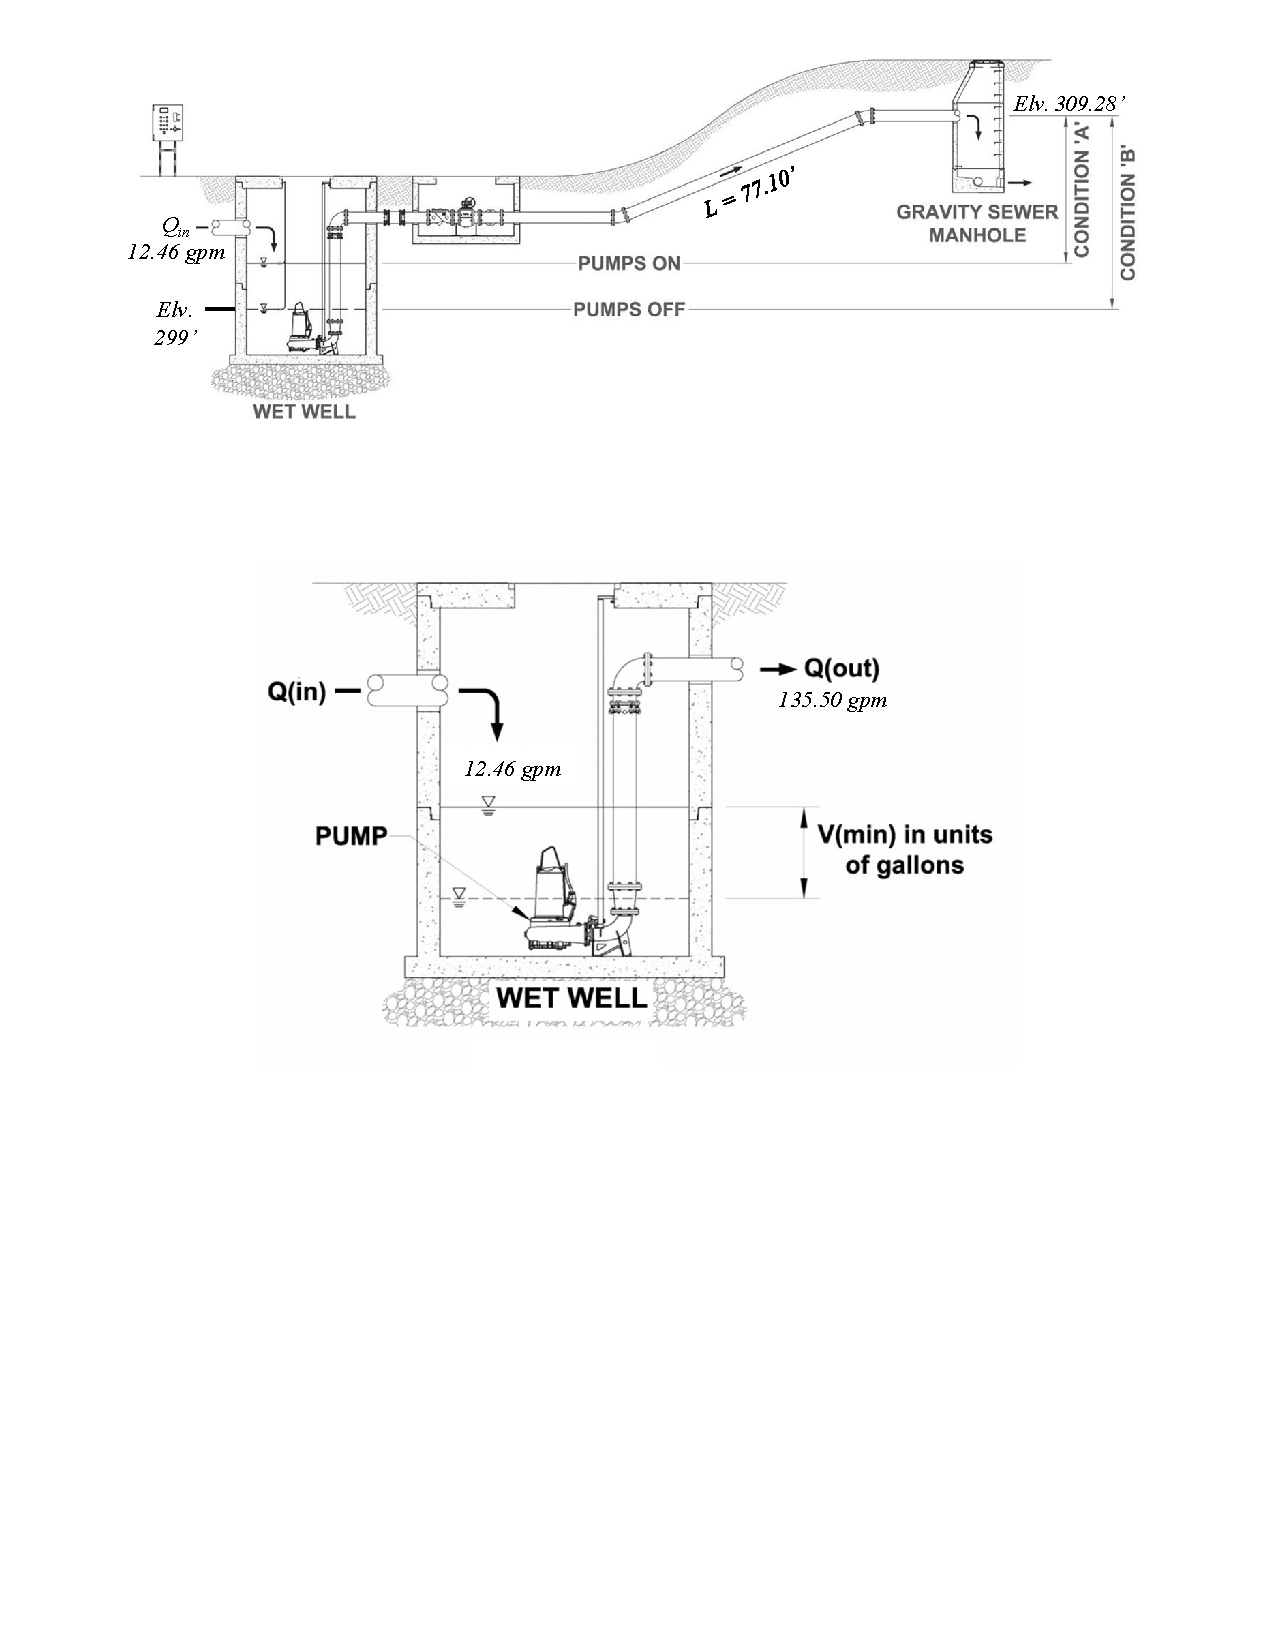
\includegraphics[
        page=1,
        width=\textwidth,
        trim={0.1in 8.0in 0.1in 0.1in},
        clip
    ]{forcemain_pump_figures.pdf}
    \caption{Pump station and force main profile showing wet well elevation, discharge elevation, and force main alignment.}
    \label{fig:force_main_profile}
\end{figure}

As illustrated in Figure~\ref{fig:force_main_profile}, the force main discharges to a gravity sewer manhole rather than to a pressurized system. Therefore, the static head is controlled only by the elevation difference between the receiving manhole invert and the wet well water surface. Jensen also notes that this value is not strictly fixed during operation because the wet well water surface fluctuates between the pumps-on and pumps-off elevations~\cite{Jensen_PumpStationDesignGuidelines_2012}. For conservative design and preliminary hydraulic analysis, the pumps-off elevation is used here, which produces the maximum static head condition.

The static head determined in this section forms the first component of the total dynamic head. The next step is to evaluate the friction losses that occur in the 4-in PVC force main during wastewater conveyance.

% -------------------------------------------------
% 3.4 Friction Loss in the Force Main
% -------------------------------------------------
\subsection{Friction Loss in the Force Main}

Dynamic losses in a pumping system arise primarily from friction as wastewater flows through the force main and associated fittings. Unlike static head, which is controlled by elevation difference, friction losses increase with flow rate and depend on the pipe material, pipe diameter, and internal flow conditions. Several methods exist to estimate friction losses in pressurized pipelines, including the Darcy--Weisbach equation and the Hazen--Williams equation. For wastewater lift station applications involving a simple force main discharging to gravity, the Hazen--Williams formulation is commonly adopted because it provides a relatively straightforward method for estimating friction losses while maintaining acceptable engineering accuracy~\cite{Jensen_PumpStationDesignGuidelines_2012}. In addition, many regulatory agencies allow or require the Hazen--Williams method for wastewater force main design~\cite{MDEQ_DesignGuidance_2025}.

The Hazen--Williams equation is applicable under turbulent flow conditions and is most reliable when velocities fall within a practical operating range. Jensen notes that velocities between approximately $3$ and $9~\text{ft/s}$ are desirable for wastewater force mains. Velocities below this range may allow solids to settle in the pipeline, while excessively high velocities can cause pipe abrasion or structural damage. These limits therefore provide a useful guideline when evaluating pump discharge conditions and developing the system curve for the force main~\cite{Jensen_PumpStationDesignGuidelines_2012}.

For this design, the friction-loss calculation will be based on a $4$-in PVC force main, a Hazen--Williams coefficient of $C = 135$, a force main length of $L = 77.48~\text{ft}$, and an initial inflow of $Q = 12.46~\text{gpm}$. These values are used because they correspond to the selected preliminary pipe material and diameter and the site layout established for the Colebrooke Subdivision system. A detailed sample calculation will be presented later with the system-curve development.

\pagebreak
The base form of the Hazen--Williams equation is written as

\begin{equation}
v = 1.318\, C\, R^{0.63} S^{0.54}
\end{equation}


where

$v$ = velocity ($\text{ft/s}$), 

$C$ = Hazen--Williams friction coefficient, 

$R$ = hydraulic radius ($\text{ft}$), 

$S$ = headloss slope ($\text{ft/ft}$)

For force main design, the conventional rearranged form used to estimate friction headloss is

\begin{equation}
h_f = 10.5\, L \left(\frac{Q}{C}\right)^{1.85} D^{-4.87}
\end{equation}

where

$h_f$ = friction headloss ($\text{ft}$)

$L$ = force main length ($\text{ft}$)

$Q$ = flow rate ($\text{gpm}$)

$C$ = Hazen--Williams friction coefficient ($-$)

$D$ = pipe diameter ($\text{in}$)

For PVC pipe, Jensen reports a wastewater design coefficient range of approximately $130$ to $145$, and the adopted value of $C = 135$ falls within this recommended range and also satisfies MDEQ guidelines.~\cite{Jensen_PumpStationDesignGuidelines_2012, MDEQ_DesignGuidance_2025}. Using the selected design parameters, the friction headloss for the $4$-in PVC force main at the initial inflow condition is very small relative to the static head because of the short pipe length and low flow rate. This friction component will be combined with static and minor losses in the following subsection to determine the total dynamic head of the system.


% -------------------------------------------------
% 3.5 Minor Loss Calculation
% -------------------------------------------------
\subsection{Minor Loss Calculation}

In addition to pipe-friction losses, the force main system also experiences localized energy losses as wastewater passes through fittings, valves, bends, and the discharge outlet. These localized losses are referred to as minor losses. Jensen notes that minor losses may be estimated either by the equivalent-length method or by using $K$-value coefficients assigned to individual fittings and appurtenances. For this project, the $K$-value method is adopted because it is straightforward and appropriate for a simple lift-station force main~\cite{Jensen_PumpStationDesignGuidelines_2012}.

Minor loss head is calculated using the following expression:

\begin{equation}
h_m = \sum K \frac{v^2}{2g}
\end{equation}



where

$h_m$ = minor headloss (ft)

$K$ = loss coefficient for each fitting or appurtenance ($-$)

$v$ = velocity of flow in the pipe (ft/s)

$g$ = gravitational acceleration ($32.2~\text{ft/s}^2$)

Based on the force main layout and coefficient values referenced from Jensen, the adopted minor-loss components include an entrance loss, one $90^\circ$ bend, one check valve, one valve, two $45^\circ$ bends, and the exit loss at the receiving manhole. The coefficients used in the hydraulic assessment are summarized in Table~\ref{tab:minor_losses}.

\begin{table}[H]
\centering
\caption{Minor Loss Coefficients Used in Hydraulic Assessment}
\label{tab:minor_losses}
\begin{tabular}{lccc}
\toprule
\textbf{Minor Loss Component} & \textbf{$K$} & \textbf{Number of Fittings} & \textbf{Sum $K$} \\
\midrule
Entrance & 0.25 & 1 & 0.25 \\
$90^\circ$ elbow & 0.25 & 1 & 0.25 \\
Check valve & 2.20 & 1 & 2.20 \\
Valve & 1.00 & 1 & 1.00 \\
$45^\circ$ bend & 0.18 & 2 & 0.36 \\
Exit & 1.00 & 1 & 1.00 \\
\midrule
 &  &  & $\Sigma K = 5.10$ \\
\bottomrule
\end{tabular}
\end{table}

Accordingly, the total minor-loss coefficient adopted for the system is

\[
\begin{aligned}
\sum K &= 5.10
\end{aligned}
\]

This value will be used together with the pipe velocity in the subsequent system-head calculations to determine the minor-loss component of the total dynamic head. A detailed sample computation of $h_m$ will be presented later with the system-curve development.


% -------------------------------------------------
% 3.6 Total Dynamic Head and System Curve
% -------------------------------------------------
\subsection{Total Dynamic Head and System Curve}

The total dynamic head (TDH) represents the total head that the pump must overcome to convey wastewater from the wet well to the downstream gravity sewer manhole. In a submersible lift station, TDH is the sum of the static head, the friction headloss in the force main, and the minor losses associated with bends, valves, and discharge conditions~\cite{Jensen_PumpStationDesignGuidelines_2012}. Jensen emphasizes that the system curve is the most important basis for pump selection because it defines the relationship between flow and the head required by the system. Rather than relying on approximate or assumed losses, TDH should be calculated at several flow rates so that the system curve can be developed and matched against candidate pump curves~\cite{Jensen_PumpStationDesignGuidelines_2012}.

The total dynamic head is expressed as

\[
\begin{aligned}
TDH &= \Delta H + h_f + h_m
\end{aligned}
\]

where

\begin{itemize}
\item $TDH$ = total dynamic head (ft)
\item $\Delta H$ = static head (ft)
\item $h_f$ = friction headloss (ft)
\item $h_m$ = minor headloss (ft)
\end{itemize}

Substituting the friction-loss and minor-loss expressions gives

\[
\begin{aligned}
TDH &= \Delta H 
+ (L)\,10.5\left(\frac{Q}{C}\right)^{1.85}D^{-4.87}
+ \Sigma K \frac{v^2}{2g}
\end{aligned}
\]

For the Colebrooke Subdivision pump station, the parameters used for the system-curve development are

\[
\begin{aligned}
\Delta H &= 10.28\ \text{ft} \\
D &= 4.00\ \text{in} \\
A &= 0.09\ \text{ft}^2 \\
C &= 135 \\
\Sigma K &= 5.10 \\
L &= 77.48\ \text{ft}
\end{aligned}
\]

Using these values, TDH was calculated for a range of discharge flow rates. The results are summarized in Table~\ref{tab:system_curve}.

\begin{table}[H]
\centering
\caption{System Curve Calculation for 4-in PVC Force Main}
\label{tab:system_curve}
\begin{tabular}{ccccccc}
\toprule
\textbf{Flow} & \textbf{Flow} & \textbf{Velocity} & \textbf{$h_m$} & \textbf{$h_f$} & \textbf{$\Delta H$} & \textbf{TDH} \\
(gpm) & (cfs) & (ft/s) & (ft) & (ft) & (ft) & (ft) \\
\midrule
0   & 0.00 & 0.0 & 0.00 & 0.0 & 10.28 & 10.3 \\
20  & 0.04 & 0.5 & 0.02 & 0.0 & 10.28 & 10.3 \\
40  & 0.09 & 1.0 & 0.08 & 0.1 & 10.28 & 10.5 \\
60  & 0.13 & 1.5 & 0.19 & 0.2 & 10.28 & 10.7 \\
80  & 0.18 & 2.0 & 0.33 & 0.4 & 10.28 & 11.0 \\
100 & 0.22 & 2.6 & 0.52 & 0.5 & 10.28 & 11.3 \\
120 & 0.27 & 3.1 & 0.74 & 0.8 & 10.28 & 11.8 \\
140 & 0.31 & 3.6 & 1.01 & 1.0 & 10.28 & 12.3 \\
160 & 0.36 & 4.1 & 1.32 & 1.3 & 10.28 & 12.9 \\
\bottomrule
\end{tabular}
\end{table}

\subsubsection*{Sample Calculation (Design Flow = 120 gpm)}

A sample calculation is shown below for a discharge flow of $120~\text{gpm}$, which is used as the design point for pump-curve evaluation.

For this system, the adopted design parameters are

\[
\begin{aligned}
\Delta H &= 10.28\ \text{ft} \\
D &= 4.00\ \text{in} = \frac{4}{12} = 0.333\ \text{ft} \\
A &= 0.09\ \text{ft}^2 \\
C &= 135 \\
\Sigma K &= 5.1 \\
L &= 77.48\ \text{ft} \\
g &= 32.2\ \text{ft/s}^2 \\
Q &= 120\ \text{gpm}
\end{aligned}
\]

\textbf{Convert flow from gpm to cfs}

\[
\begin{aligned}
Q &= 120\ \text{gpm}\times 
\frac{1\ \text{ft}^3}{7.48\ \text{gal}}\times 
\frac{1}{60\ \text{s/min}} \\
&\therefore Q = 0.267\ \text{ft}^3/\text{s}
\end{aligned}
\]

\textbf{Compute pipe velocity}

\[
\begin{aligned}
v &= \frac{Q}{A} \\
&\Rightarrow v = \frac{0.267}{0.0873} \\
&\therefore v = 3.06\ \text{ft/s}
\end{aligned}
\]

Using rounding consistent with the system-curve table,

\[
v \approx 3.1\ \text{ft/s}
\]

\textbf{Compute minor loss head}

\[
\begin{aligned}
&h_m = \Sigma K\frac{v^2}{2g} \\
&\Rightarrow h_m = 5.1\left(\frac{(3.06)^2}{2(32.2)}\right) \\
&= 5.1\left(\frac{9.36}{64.4}\right) \\
&= 5.1(0.1453) \\
&\therefore h_m = 0.741\ \text{ft}
\end{aligned}
\]

Thus,

\[
h_m \approx 0.74\ \text{ft}
\]

\textbf{Compute friction headloss}

Using the Hazen--Williams formulation adopted in this report,

\[
\begin{aligned}
&h_f = (L)10.5\left(\frac{Q}{C}\right)^{1.85}D^{-4.87} \\
&\Rightarrow h_f = (77.48)(10.5)
\left(\frac{120}{135}\right)^{1.85}(4)^{-4.87} \\
&\Rightarrow h_f = (77.48)(10.5)(0.804)(0.00117) \\
&\therefore h_f = 0.765\ \text{ft}
\end{aligned}
\]
Using rounding consistent with the system-curve table,

\[
h_f \approx 0.8\ \text{ft}
\]

\textbf{Compute total dynamic head}

\[
\begin{aligned}
TDH &= \Delta H + h_f + h_m \\
&\Rightarrow TDH = 10.28 + 0.77 + 0.74 \\
&\therefore TDH = 11.79\ \text{ft}
\end{aligned}
\]

Therefore,

\[
TDH \approx 11.8\ \text{ft}
\]

So, at a discharge flow of $120~\text{gpm}$, the system requires

\[
\boxed{TDH = 11.8\ \text{ft}}
\]

This point is used for pump-curve evaluation because it produces a force-main velocity of $3.1~\text{ft/s}$, which exceeds the MDEQ minimum velocity criterion of $2~\text{ft/s}$ and falls within the desirable wastewater transport range discussed in the Jensen guidance.

The resulting system curve is shown in Figure~\ref{fig:system_curve}

\begin{figure}[H]
\centering
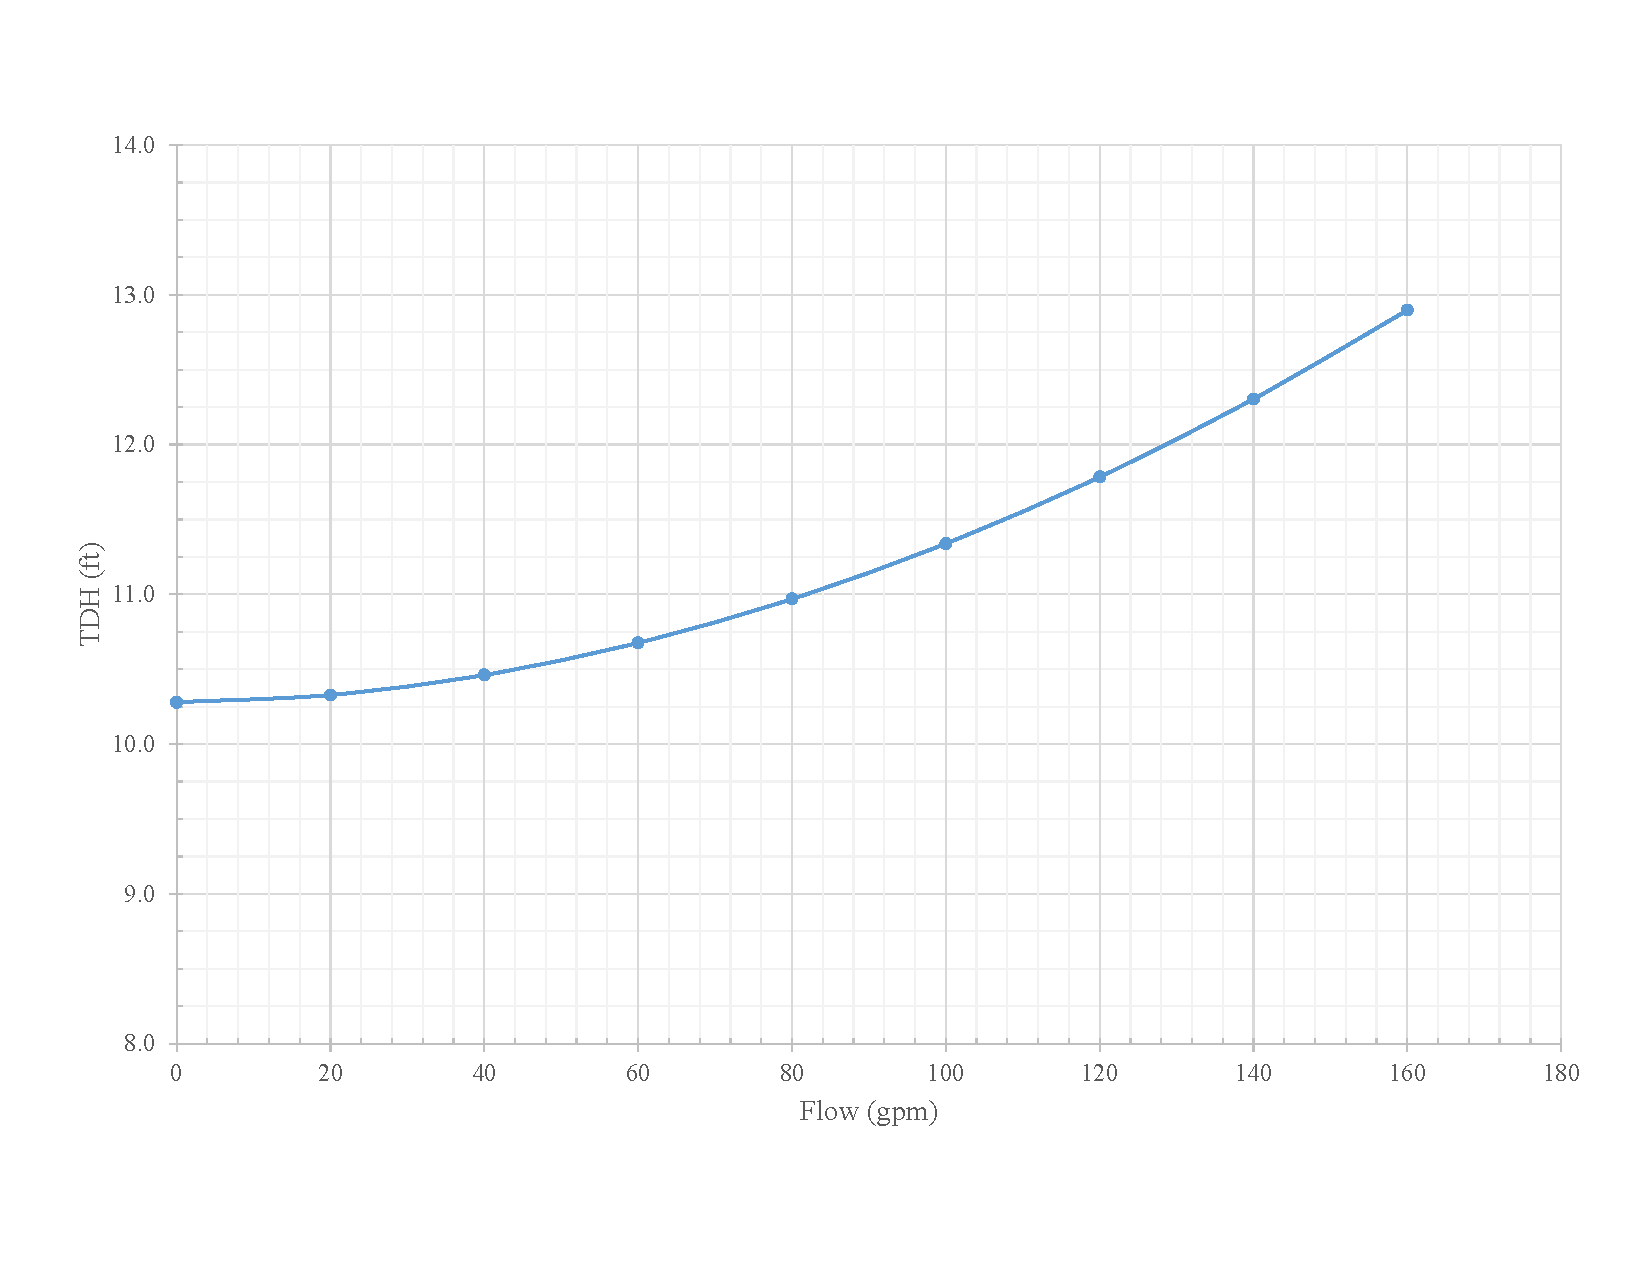
\includegraphics[
width=\textwidth,
% trim={0.2in 0.2in 0.2in 0.2in},
% clip
]{system-curve.pdf}
\caption{System curve showing total dynamic head versus flow for the 4-in PVC force main.}
\label{fig:system_curve}
\end{figure}

As shown in Figure~\ref{fig:system_curve}, the system head increases gradually with increasing flow because the static head remains constant while the friction and minor losses increase with discharge. This system curve will be used in the next section to evaluate candidate pump curves and identify an appropriate operating point for the Colebrooke Subdivision pump station.
